\documentclass{article}
\usepackage[utf8]{inputenc}
\usepackage[margin=0.6in]{geometry}
% Math
\usepackage{amsmath}
\usepackage{physics}
\usepackage{simpler-wick}
\usepackage{subcaption}

% Citetations
\usepackage[ backend=bibtex, sorting=none, autocite=plain]{biblatex}
\addbibresource{refs/references}
\usepackage{xcolor}
\usepackage{hyperref}
\hypersetup{
    colorlinks,
    linkcolor={red!50!black},
    citecolor={blue!50!black},
    urlcolor={blue!80!black}}


% Formatting
\usepackage{float}
\usepackage{graphicx}
\graphicspath{ {./figs/} } 

% Referecing sections, equations etc
\usepackage[capitalize]{cleveref}
\crefdefaultlabelformat{\textbf{#2}}
\crefname{eq}{Eq.}{Eq.}
\crefname{sec}{Sec.}{Sec.}
\crefname{app}{App.}{App.}
\crefname{fig}{Fig.}{Fig.}
\crefname{tab}{Tab.}{Tab.}
\crefdefaultlabelformat{#2#1#3}


% Misc
\usepackage{appendix}

% Commands
\newcommand{\crt}[1]{a_{#1}^{\dagger}}
\newcommand{\ani}[1]{a_{#1}}
\newcommand{\vac}{\ket{0}}
\newcommand{\gs}{\ket{\Phi_0}}
\newcommand{\exed}[2]{\ket{\Phi_{#1}^{#2}}}

\newcommand{\inner}[3]{\bra{#1}#2\ket{#3}}
\newcommand{\innerAS}[3]{\inner{#1}{#2}{#3}_{\text{AS}}}
\newcommand{\set}[1]{\{ #1 \}}
\newcommand{\ord}[2]{#1^{(#2)}}
\newcommand{\energyref}{E_0^{\text{ref}}}
\newcommand{\psum}{\sideset{}{'}\sum}

\newcommand{\spinop}[1]{\hat{S}_{#1}}
\newcommand{\pplus}[1]{\hat{P}_{#1}^{+}}
\newcommand{\pminus}[1]{\hat{P}_{#1}^{-}}
\newcommand{\numberop}[1]{\hat{N}_{#1}}
\newcommand{\hatreefock}[1]{#1^{\text{HF}}}
\newcommand{\comment}[1]{\textcolor{red}{#1}}


\title{FYS4480 Midterm 2}
\author{Håkon Kvernmoen}
\date{December 2022}

\begin{document}
\maketitle

\section*{Task 1}
We begin by defining the unperturbed Hamiltonian $\hat{H}_0$ and the perturbation $\hat{V}$, setting up the total Hamiltonian of our system $\hat{H}$. Expressed using creation and annihilation operators, we have the following:
\begin{align}
    \hat{H} = \hat{H}_0 + \hat{V},\hspace{20px} \hat{H}_0 = \xi\sum_{p\sigma} (p-1)\crt{p\sigma}\ani{p\sigma}, \hspace{20px}\hat{V} = -\frac{1}{2}g\sum_{pq}\crt{p+}\crt{p-}\ani{q-}\ani{q+} \label[eq]{eq:hamiltonian}
\end{align}
Here, $\hat{H}_0$ is a one body operator, and $\hat{V}$ a two body operator. We define pair creation and pair annihilation operators, either adding a pair of particles in energy state $p$ with opposite spins, or annihilation a pair in state $p$ with opposite spins. One thing to notice is that these operators are hermitian conjugates of each other.

\begin{align}
    \pplus{p} = \crt{p+} \crt{p-},\hspace{20px}\pminus{p} = \ani{p-}\ani{p+},\hspace{20px}\pplus{p} = (\pminus{p})^\dagger \label[eq]{eq:pair_crt_and_ani}
\end{align}
Substituting these in for the perturbation $\hat{V}$ in \cref{eq:hamiltonian}, we get:

\begin{align}
    \hat{V} = -\frac{1}{2}g\sum_{pq} \pplus{p} \pminus{q} \label[eq]{eq:V_pair_operators}
\end{align}
We also define a component of the number operator $\numberop{p\sigma} = \crt{p\sigma}\ani{p\sigma}$, giving one if the state contains $p\sigma$, zero else. Setting $\xi = 1$, the total Hamiltonian becomes:

\begin{align}
    \hat{H} = \sum_{p\sigma} (p-1)\numberop{p\sigma} -\frac{1}{2}g\sum_{pq} \pplus{p} \pminus{q} \label[eq]{eq:H_pair_operators}
\end{align}
Moving on, we define the spin projection along the $z$ axis $\spinop{z}$, spin ladder operators $\spinop{\pm}$ and the total squared spin of the system $\spinop{}^2$ as: 

\begin{align}
    \spinop{z} = \frac{1}{2} \sum_{p\sigma} \sigma \crt{p\sigma}\ani{p\sigma} = \frac{1}{2}\sum_{p\sigma} \sigma \numberop{p\sigma},\hspace{20px} \spinop{\pm} = \sum_p \crt{p\pm}\ani{p\mp}\hspace{20px}\spinop{}^2 = \spinop{z}^2 + \frac{1}{2}\left( \spinop{+}\spinop{-} + \spinop{-}\spinop{+}\right) \label[eq]{eq:spin_operators}
\end{align}
We begin by calculating some commutators, beginning with $[\hat{H}_0, \spinop{z}]$. Both these operators consists of the operator $\numberop{p\sigma}$, which of course should commute:   

\begin{align*}
    \numberop{p\sigma}\numberop{q\tau} &= \crt{p\sigma}\ani{p\sigma}\crt{q\tau}\ani{q\tau} = \crt{p\sigma} (\delta_{pq}\delta_{\sigma\tau} - \crt{q\tau}\ani{p\sigma})a_{q\tau} = \delta_{pq}\delta_{\tau\sigma}\crt{p\sigma}\ani{q\tau} - \crt{q\tau}\crt{p\sigma}\ani{q\tau}\ani{p\sigma} \\
    &= \delta_{pq}\delta_{\tau\sigma}\crt{p\sigma}\ani{q\tau} - \delta_{pq}\delta_{\tau\sigma}\crt{q\tau}\ani{p\sigma} + \crt{q\tau}\ani{q\tau}\crt{p\sigma}\ani{p\sigma} = \numberop{q\tau}\numberop{p\sigma}
\end{align*}
It is now easy to show that the $[\hat{H}_0, \spinop{z}]$ commutator becomes:

\begin{align}
    [\hat{H_0}, \spinop{z}] = \frac{1}{2}\sum_{p\sigma q\tau} (p-1)\tau [\numberop{p\sigma}, \numberop{q\tau}] = 0 \label[eq]{eq:commutator_Hnull_Sz}
\end{align}
Next, we want to calculate $[\hat{V}, \spinop{z}]$. $\hat{V}$ contains the product of $\pplus{p}$ and $\pplus{q}$, while $\spinop{z}$ again contains a $\numberop{p\sigma}$. Finding the commutator of the operators inside the sum then yields for $[\pplus{p}, \spinop{z}]$:  

\begin{align*}
    \pplus{p} \numberop{q\sigma} &= \crt{p+}\crt{p-}\crt{q\sigma}\ani{q\sigma} = \crt{q\sigma}\crt{p+}\crt{p-}\ani{q\sigma} = \crt{q\sigma}\crt{p+}(\delta_{pq}\delta_{\sigma-} - \ani{q\sigma}\crt{p-}) \\
    &= -\delta_{pq}\delta_{\sigma-}\crt{p+}\crt{q\sigma} -\delta_{pq}\delta_{\sigma+}\crt{q\sigma}\crt{p-} + \crt{q\sigma}\ani{q\sigma}\crt{p+}\ani{p-} \\
    &= -\delta_{pq}\delta_{\sigma-}\crt{p+}\crt{q\sigma} -\delta_{pq}\delta_{\sigma+}\crt{q\sigma}\crt{p-} + \numberop{q\sigma}\pplus{p} \\
    \Rightarrow& [\pplus{p},\numberop{q\sigma}] = -\delta_{pq}\delta_{\sigma-}\crt{p+}\crt{q\sigma} -\delta_{pq}\delta_{\sigma+}\crt{q\sigma}\crt{p-}\\
    \Rightarrow& [\pplus{p}, \spinop{z}] = \frac{1}{2}\sum_{q\sigma} \sigma[\pplus{p}, \numberop{q\sigma}] = -\frac{1}{2}\sum_{q\sigma} \sigma \left(\delta_{pq}\delta_{\sigma-}\crt{p+}\crt{q\sigma} +\delta_{pq}\delta_{\sigma+}\crt{q\sigma}\crt{p-} \right) = -\frac{1}{2}\left( - \crt{a+}\crt{a-} + \crt{a+}\crt{a-} \right) = 0
\end{align*}
Since $\spinop{z}$ is hermitian and  $\pplus{p} = (\pminus{p})^\dagger$, this results also gives us $[\pminus{p},\spinop{z}] = 0$.

\begin{align*}
    [\pplus{p}, \spinop{z}]^\dagger = (\pplus{p}\spinop{z})^\dagger - (\spinop{z}\pplus{p})^\dagger = \spinop{z}\pminus{p} - \pminus{p}\spinop{z} = -[\pminus{p}, \spinop{z}] = 0
\end{align*}
Now, calculating $[\hat{V}, \spinop{z}]$ follows:

\begin{align}
    [\hat{V}, \spinop{z}] = -\frac{1}{2}g \sum_{pq} [\pplus{p}\pminus{q},\spinop{z}] = -\frac{1}{2}g \sum_{pq} \pplus{p}[\pminus{q}, \spinop{z}] + [\pplus{p},\spinop{z}]\pminus{q} = 0 \label[eq]{eq:commutator_V_Sz}
\end{align}
We now move on to calculating $[\hat{H}_0, \spinop{}^2]$. $\spinop{}^2$ contains the operators $\spinop{z}$, $\spinop{+}$ and $\spinop{-}$. The commutator with $\spinop{z}$ has already been found to be zero, thus finding $[\hat{H}_0, \spinop{\pm}]$:

\begin{align*}
    \numberop{p\sigma}\crt{q+}\ani{q-} &= \crt{p\sigma}\ani{p\sigma}\crt{q+}\ani{q-} = \crt{p\sigma}(\delta_{pq}\delta_{\sigma+} - \crt{q+}\ani{p\sigma})\ani{q-} = \delta_{pq}\delta_{\sigma+} \crt{p\sigma}\ani{q-} - \crt{q+}\crt{p\sigma}\ani{q-}\ani{p\sigma} \\
    &= \delta_{pq}\delta_{\sigma+} \crt{p\sigma}\ani{q-} - \delta_{pq}\delta_{\sigma-} \crt{q+}\ani{p\sigma} + \crt{q+}\crt{q-}\crt{p\sigma}\ani{p\sigma} \\
    &= \delta_{pq}\delta_{\sigma+} \crt{p\sigma}\ani{q-} - \delta_{pq}\delta_{\sigma-} \crt{q+}\ani{p\sigma} + \crt{q+}\crt{q-}\numberop{p\sigma} \\
    \Rightarrow& [\numberop{p\sigma}, \crt{q+}\ani{q-}] = \delta_{pq}\delta_{\sigma+} \crt{p\sigma}\ani{q-} - \delta_{pq}\delta_{\sigma-} \crt{q+}\ani{p\sigma} \\
    \Rightarrow& [\hat{H}_0, \spinop{+}] = \sum_{pq\sigma} (p-1) [\numberop{p\sigma}, \crt{q+}\ani{q-}] = \sum_{pq\sigma} (p-1)(\crt{p+}\ani{p-}-\crt{p+}\ani{p-}) = 0
\end{align*}
Since $\hat{H}_0$ is hermitian and $\spinop{+} = (\spinop{-})^\dagger$, we can use this results to conclude that $[\hat{H}_0, \spinop{-}] = 0$:

\begin{align*}
    [\hat{H}_0, \spinop{+}]^\dagger = \spinop{-}\hat{H}_0 - \hat{H}_0 \spinop{-} = -[\hat{H}_0, \spinop{-}] = 0
\end{align*}
Now using the expression for $\spinop{}^2$ (\cref{eq:spin_operators}) in addition to $[\hat{H}_0, \spinop{z}] = [\hat{H}_0, \spinop{+}] = [\hat{H}_0, \spinop{-}] = 0$ we calculate the commutator as:

\begin{align}
    [\hat{H}_0, \spinop{}^2] &= [\hat{H}_0, \spinop{z}^2] + \frac{1}{2}\left( [\hat{H_0}, \spinop{+}\spinop{-}] + [\hat{H_0}, \spinop{-}\spinop{+}]\right) \nonumber\\
    &= [\hat{H}_0, \spinop{z}]\spinop{z} + \spinop{z}[\hat{H}_0, \spinop{z}] + \frac{1}{2}\left( [\hat{H}_0, \spinop{+}]\spinop{-} + \spinop{+}[\hat{H}_0, \spinop{-}] + [\hat{H}_0, \spinop{-}]\spinop{+} + \spinop{-}[\hat{H}_0, \spinop{+}] \right) = 0 \label[eq]{eq:commutator_Hnull_S2}
\end{align}
Moving on to $[\hat{V}, \spinop{}^2]$, again to commutator with $\spinop{z}$ has already been found. Therefor, we only need to find $[\hat{V}, \spinop{\pm}]$. Again, since $\hat{V}$ contains the pair creation operators $\hat{P}_p^{\pm}$, $[\hat{P}_p^{\pm}, \spinop{\pm}]$ will help us find the total results. We begin with $[\pplus{q}, \spinop{+}]$:

\begin{align*}
    \pplus{p}\crt{q+}\ani{q-} &= \crt{p+}\crt{p-}\crt{q+}\ani{q-} = \crt{q+}\crt{p+}\crt{p-}\ani{q-} = \crt{q+}\crt{p+}(\delta_{pq} - \ani{q-}\crt{p-}) = \delta_{pq}\crt{q+}\crt{p+} + \crt{q+}\crt{q-}\pplus{p} \\
    [\pplus{p}, \crt{q+}\ani{q-}] &= \delta_{pq}\crt{q+}\crt{p+} \\
    [\pplus{p}, \spinop{+}] &= \sum_q [\pplus{p}, \crt{q+}\ani{q-}] = \sum_q \delta_{pq}\crt{q+}\crt{p+} = \crt{p+}\crt{p+} = 0
\end{align*}
Similarly for $[\pplus{q}, \spinop{-}]$:

\begin{align*}
    \pplus{p}\crt{q-}\ani{q+} &= \crt{p+}\crt{p-}\crt{q-}\ani{q+} = -\crt{q-}\crt{p+}\ani{q+}\crt{p-} = -\crt{q-}(\delta_{pq} - \ani{q+}\crt{p+})\crt{p+} = \delta_{pq}\crt{p-}\crt{q-} + \crt{q-}\ani{q+}\pplus{p} \\
    [\pplus{p}, \crt{q-}\ani{q+}] &= \delta_{pq} \crt{p-}\crt{q-} \\
    [\pplus{p}, \spinop{-}] &= \sum_q [\pplus{p}, \crt{q-}\ani{q+}] = \sum_q \delta_{pq} \crt{p-}\crt{q-} = \crt{p-}\crt{p-} = 0
\end{align*}
These results can also be used for the two other commutators:
\begin{align*}
    [\pplus{+}, \spinop{+}]^\dagger &= \spinop{-}\pminus{p} - \pminus{p}\spinop{-} = -[\pminus{p},\spinop{-}] = 0 \\
    [\pplus{+}, \spinop{-}]^\dagger &= \spinop{+}\pminus{p} - \pminus{p}\spinop{+} = -[\pminus{p},\spinop{+}] = 0
\end{align*}
Collectively giving:

\begin{align*}
    [\hat{V}, \spinop{\pm}] = -\frac{1}{2}g\sum_{pq} [\pplus{p}\pminus{q}, \spinop{\pm}] = -\frac{1}{2}g \sum_{pq} \pplus{p}[\pminus{q}, \spinop{\pm}] + [\pplus{p}, \spinop{\pm}]\pminus{q} = 0
\end{align*}
Then, through the same procedure as in \cref{eq:commutator_Hnull_S2}, the perturbation Hamiltonian and spin squared commutator becomes:

\begin{align}
    [\hat{V}, \spinop{}^2] = 0 \label[eq]{eq:commutator_V_S2}
\end{align}
Finally *sigh*, the last commutator we will look at is between the pair creation and annihilation operators, $[\hat{P}^{\pm}_p, \hat{P}^{\pm}_q]$. This one is quite easy, as it contains only creation or only annihilation operators. Explicitly for the pair creation operators:

\begin{align*}
    \pplus{p}\pplus{q} &= \crt{p+}\crt{p-}\crt{q+}\crt{q-} = (-1)^4 \crt{q+}\crt{q-}\crt{p+}\crt{p-} = \pplus{q}\pplus{p} \\
    [\pplus{p}, \pplus{q}] &= 0 \\
\end{align*}
Which, through its complex conjugate gives the pair annihilation commutator.
\begin{align*}
    [\pminus{p}, \pminus{q}] &= - [\pplus{p}, \pplus{q}]^\dagger = 0
\end{align*}


\section*{Task 2}
    We limit ourselves to only consider the space spanned by the four energy levels $p = 1,2,3,4$. In addition, all states created must have total spin $S = 0$ in addition to containing no broken pairs (that is, if for instance the state $\ket{p\sigma} = \ket{2+}$ is occupied, we must also include $\ket{2-}$). By considering a system of four particles, the obvious ansatz for our ground state then becomes:
    
    \begin{align*}
        \gs = \ket{12} = \crt{1+}\crt{1-}\crt{2+}\crt{2-}\vac = \pplus{1}\pplus{2} \vac
    \end{align*}
    Where, since no broken pairs are allowed, the usefulness of the pair creation and annihilation operators becomes apparent. The notation $\ket{12}$ here does not mean a two particle state, but a two pair state (and therefor a four particle states). When the pairs are not specified, large letters will be used (i.e. $\ket{PQ} = \ket{(p+)(p-)(q+)(q-)}$) and small letters when we refer to single particles, again with oppositely paired spin $\ket{pq} = \ket{(p+)(q-)}$. When appropriate, the spin quantum number will also be expanded. Due to no broken pairs, the only allowed excited states in this $p = 1,2,3,4$ space are 2-particle 2-holes (2p2h) excitations and 4p4h excited states of $\gs$. This yields five possible excited states:

    \begin{align*}
        \ket{13} = \pplus{1}\pplus{3}\vac, \ket{14} = \pplus{1}\pplus{4}\vac, \ket{23} = \pplus{2}\pplus{3}\vac, \ket{24} = \pplus{2}\pplus{4}\vac, \ket{34} = \pplus{3}\pplus{4}\vac
    \end{align*}
    Where $\ket{34}$ is the 4p4h state and the others 2p2h. In general, we have a four particle states $\ket{RS} = \pplus{r}\pplus{s}\vac$. The contribution from $\hat{H}_0$ can be calculated:
    
    \begin{align}
        \bra{KL}\hat{H}_0\ket{RS} = \sum_{p\sigma} (p-1) \bra{KL}\numberop{p\sigma}\ket{RS} = 2\sum_{p}(p-1)\bra{KL}\numberop{p}\ket{RS} = 2\sum_p (p-1) (\delta_{pr} + \delta_{ps}) \bra{KL}\ket{RS} \label[eq]{eq:task2_H0_underway} 
    \end{align}
    When calculating $\bra{KL}\ket{RS}$ using Wicks theorem, we note that (as we expect):
    
    \begin{align*}
        \bra{KL}\ket{RS} &= \bra{0} \ani{l-}\ani{l+}\ani{k-}\ani{k+}\crt{r+}\crt{r-}\crt{s+}\crt{s-}\ket{0} \\
        &= \bra{0} \wick{ \c4{\ani{l-}} \c3{\ani{l+}} \c2{\ani{k-}} \c1{\ani{k+}}\c1{a}_{r+}^\dagger \c2{a}_{r-}^\dagger \c3{a}_{s+}^\dagger \c4{a}_{s-}^\dagger }\ket{0} + \bra{0} \wick{ \c4{\ani{l-}} \c3{\ani{l+}} \c2{\ani{k-}} \c1{\ani{k+}}\c3{a}_{r+}^\dagger \c4{a}_{r-}^\dagger \c1{a}_{s+}^\dagger \c2{a}_{s-}^\dagger }\ket{0} = \delta_{kr}\delta_{ls} + \delta_{ks}\delta_{lr}
    \end{align*}
    However, due to the states always consisting of antiparallel pair states, we can use $\pplus{}$ and $\pminus{}$ in the same manner, but now without a minus sign for an odd number of crossing lines (noting the almost bosonic commutation relations). This can be demonstrated by:
    
    \begin{align*}
        \bra{KL}\ket{RS} = \bra{0} \wick{ \c3{\pminus{l}} \c2{\pminus{k}} \c2{\pplus{r}} \c3{\pplus{s}} } \ket{0} + \bra{0} \wick{ \c3{\pminus{l}} \c2{\pminus{k}} \c3{\pplus{r}} \c2{\pplus{s}} } \ket{0} = \delta_{kr}\delta_{ls} + \delta_{ks}\delta_{lr}
    \end{align*}
    Moving on from this little digression, we insert this into the matrix elements for $\hat{H}_0$ (\cref{eq:task2_H0_underway}) giving:

    \begin{align}
        \inner{KL}{\hat{H}_0}{RS} = 2\left( r+s-2\right) \left( \delta_{kr}\delta_{ls} + \delta_{ks}\delta_{lr} \right) \label[eq]{eq:task2_H0_done}
    \end{align}
    Which clearly only contributes on the diagonal. Now, the same procedure for $\hat{V}$ (\cref{eq:V_pair_operators}) gives: 

    \begin{align}
        \bra{KL}\hat{V} \ket{RS} &= -\frac{1}{2}g\sum_{pq}\inner{0}{\pminus{l}\pminus{k}\pplus{p}\pminus{q}\pplus{r}\pplus{s}}{0} \nonumber \\
        &= -\frac{1}{2}g\sum_{pq} \Big( \inner{0}{ \wick{\c3{\pminus{l}}\c2{\pminus{k}}\c2{\pplus{p}}\c2{\pminus{q}}\c2{\pplus{r}}\c3{\pplus{s}}} }{0} + \inner{0}{ \wick{\c3{\pminus{l}}\c2{\pminus{k}}\c2{\pplus{p}}\c2{\pminus{q}}\c3{\pplus{r}}\c2{\pplus{s}}} }{0} \nonumber \\
        &+ \inner{0}{ \wick{\c2{\pminus{l}}\c3{\pminus{k}}\c2{\pplus{p}}\c2{\pminus{q}}\c2{\pplus{r}}\c3{\pplus{s}}} }{0} + \inner{0}{ \wick{\c2{\pminus{l}}\c3{\pminus{k}}\c2{\pplus{p}}\c2{\pminus{q}}\c3{\pplus{r}}\c2{\pplus{s}}} }{0} \Big) \nonumber \\
        &= -\frac{1}{2}g\sum_{pq} \Big( \delta_{ls}\delta_{kp}\delta_{qr} + \delta_{qs}\delta_{kp}\delta_{lr} + \delta_{lp}\delta_{ks}\delta_{qr} + \delta_{lp}\delta_{kr}\delta_{qs} \Big) \nonumber \\
        &= -\frac{1}{2}g \Big( \delta_{ls} + \delta_{lr} + \delta_{ks} + \delta_{kr} \Big) \label[eq]{eq:task2_V_done}
    \end{align}
    Now with these matrix elements at hand, we have everything we need to construct the $6 \times 6$ Hamiltonian matrix. These results will be referred to as the exact solutions, since in our limited space this corresponds to full configuration interaction (FCI). The chosen ordering follows (column wise): $\ket{12}, \ket{13}, \ket{14}, \ket{23}, \ket{24}, \ket{34}$, with corresponding energies $E_0, \ldots, E_5$ respectively. The energies for $g \in [-1,1]$ are presented in \cref{fig:FCI}. We see that the ground state decreases when $g \xrightarrow{} 1$, while it increases for $g \xrightarrow{} -1$. In the middle, for $g = 0$, we of course arrive back at the non-interacting case where the energy is given by the sum of the single particle energies (and our ground state ansatz is exact). 


    \begin{figure}[H]
        \centering
        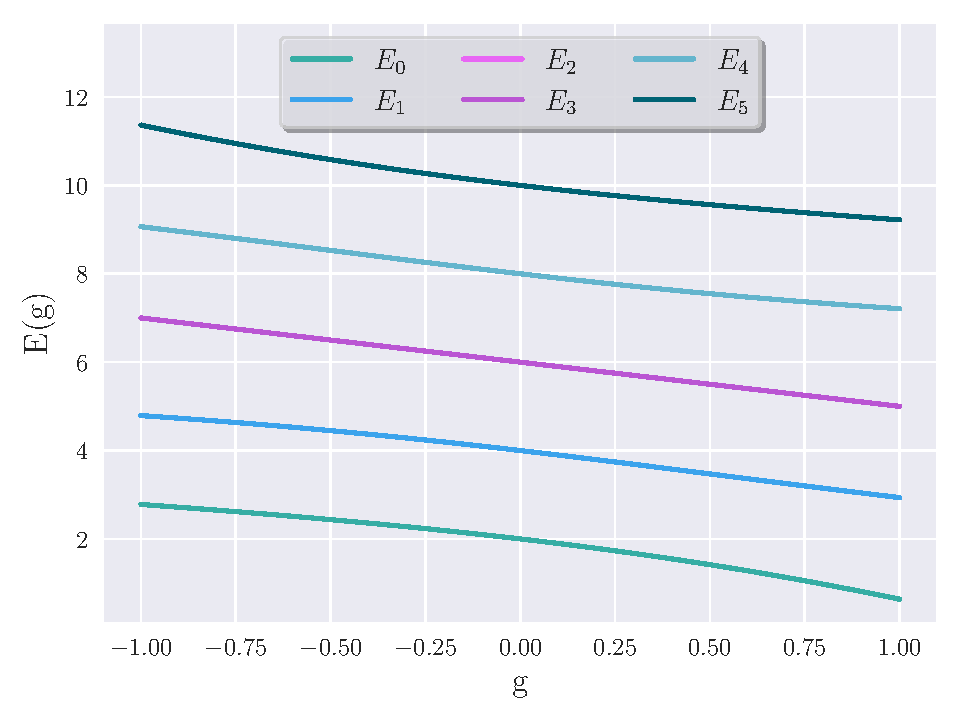
\includegraphics[width=0.7\columnwidth]{FCI.pdf}
        \caption{FCI energies for the six different states as a function of coupling strength $g$, with $E_0$ as the ground state energy. We note that $E_2$ and $E_3$ are degenerate.}
        \label[fig]{fig:FCI}
    \end{figure}
    
\section*{Task 3}
    We now aim to see how these calculations hold when we only include states up to 2p2h. This means removing the single 4p4h $\ket{34}$ state. This shrinks the Hamiltonian to a $5 \times 5$ matrix. The same ordering of states was used for FCI, but of course with the 4p4h contribution removed. The resulting energies for $g \in [-1,1]$ can be seen in \cref{fig:CID}. Limiting ourselves to the ground state, the absolute difference between the CID and FCI calculations are shown in \cref{fig:FCI_CID_diff}. Qualitatively the energy differences between $FCI$ and $CI$ is rather low. The $E_2$ and $E_3$ states are no longer degenerate, in comparison to what we found for FCI. The absolute difference is of course equal when $g=0$, since this corresponds to the non-interacting case. When moving away from $g = 0$, we see that the difference increases with $g$, both in the $g > 0$ and $g < 0$ case, as would be expected. However, it is not symmetric around $g = 0$, where the energy differs more in the $g > 0$ case. I have not found a concrete reason for this, but I speculate that the 4p4h coefficient would be larger in the $g > 0$ case, since both pairs are pushed into higher energy states.  
    
    The matrix elements for both the FCI and CI case looks something like what is presented in \cref{fig:task3_diagram}. Since there are no contributions from $\inner{IJ}{V}{34}$ where $\ket{IJ}$ is 2p2h, this approximation is equal to neglecting the terms where $r,k,l,s$ are \textit{all} larger than 2.  

    \begin{figure}[H]
        \begin{subfigure}{.49\textwidth}
            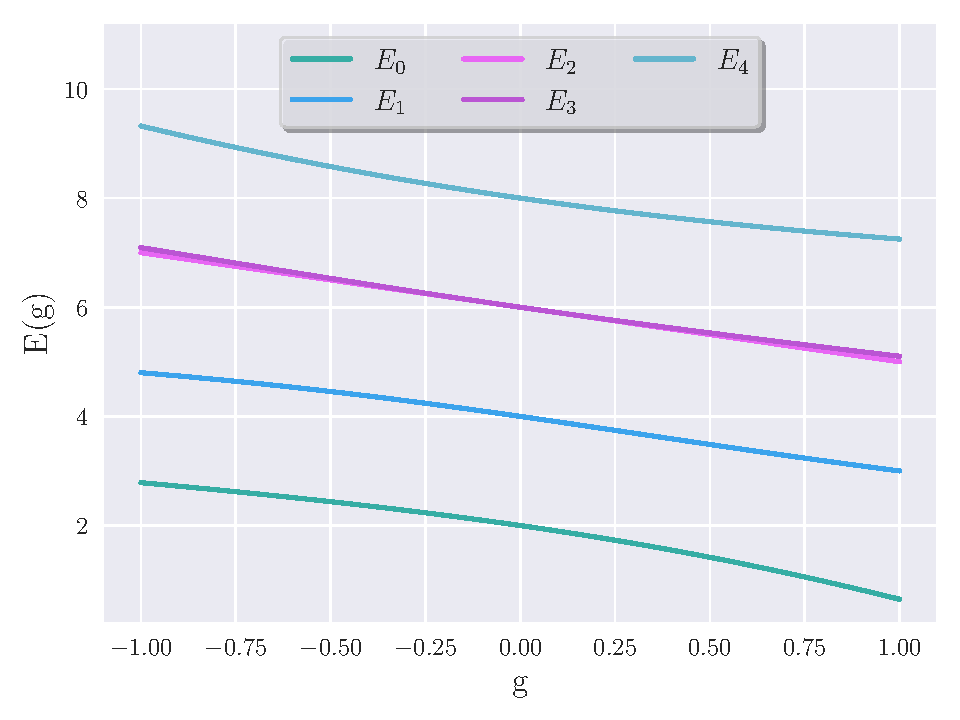
\includegraphics[width=\linewidth]{CID.pdf}
            \caption{CID energies for the five different states as a function of coupling strength $g$, with $E_0$ as the ground state energy.}
        \label[fig]{fig:CID}
        \end{subfigure}
        \hfill
        \begin{subfigure}{.49\textwidth}
            \centering
            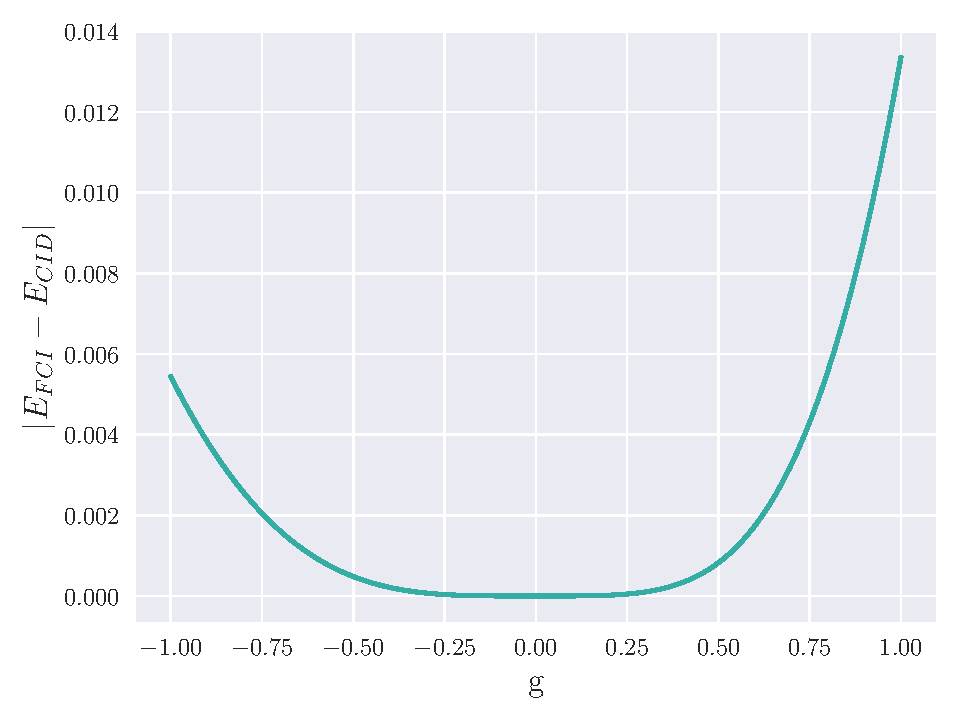
\includegraphics[width=\linewidth]{FCI_CID_diff.pdf}
            \caption{Absolute difference between ground state energies calculated using FCI and CID as a function of coupling strength $g$}
            \label[fig]{fig:FCI_CID_diff}
        \end{subfigure}
    \end{figure}

    \begin{figure}[H]
        \centering
        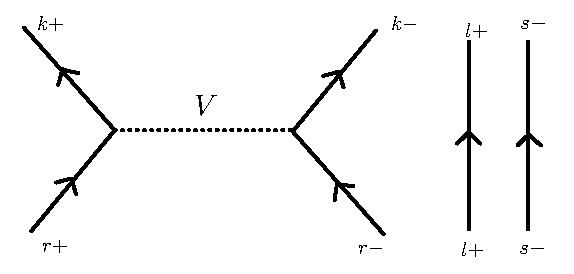
\includegraphics[width=0.6\linewidth]{task3_crop}
        \caption{The contributing matrix elements written in the particle formalism.}
        \label[fig]{fig:task3_diagram}
    \end{figure}

\section*{Task 4}
    We now aim to normal order the Hamiltonian from \cref{eq:H_pair_operators} with respect to a new reference state. Define the Fermi level to include the pairs for $p = 1, 2$ (our model space). By using the pair creation and annihilation operators on this reference state, we allow for excitations to $p = 3, 4$ (our excluded space). Since we move from the particle formalism to the particle-hole formalism, we introduce the common convention for choice of indices, where $ijk\ldots \in \set{1,2}$ indicates a state below the Fermi level and $abc\ldots \set{3,4}$ above the Fermi level. The indices $pqr\ldots$ marks an unspecified state, that can be both above and below the Fermi level $p \in \set{i,a}$. Beginning with $\hat{H}_0$ we find:

    \begin{align}
        \crt{p\sigma}\ani{p\sigma} &= \set{\crt{p\sigma}\ani{p\sigma}} + \wick{\c1{a}_{p\sigma}^\dagger \c1{a}_{p\sigma}} = \set{\crt{p\sigma}\ani{p\sigma}} + \delta_{pi} \nonumber \\
        \hat{H}_0 &= \sum_{p\sigma} (p-1) \crt{p\sigma}\ani{p\sigma} = \sum_{p\sigma} (p-1) \set{\crt{p\sigma}\ani{p\sigma}} + \sum_{i\sigma}(i-1) = \sum_{p\sigma}(p-1)\set{\numberop{p\sigma}} + 2\sum_i (i-1) \label[eq]{eq:H0_normalorder_fermi}
    \end{align}
    Similarly, for the perturbation $\hat{V}$:
    \begin{align}
        \crt{p+}\crt{p-}\ani{q-}\ani{q+} &= \set{\crt{p+}\crt{p-}\ani{q-}\ani{q+}} + \set{\crt{p+}\wick{\c1{a}_{p-}^\dagger\c1{a}_{q-}}\ani{q+}} + \set{\wick{\c1{a}_{p+}^\dagger\crt{p-}\ani{q-}\c1{a}_{q+}}} + \set{\wick{\c2{a}_{p+}^\dagger \c1{a}_{p-}^\dagger \c1{a}_{q-} \c2{a}_{q+}}} \nonumber\\
        &=  \set{\crt{p+}\crt{p-}\ani{q-}\ani{q+}} + \delta_{pi}\delta_{pq} \left(\sum_{\sigma} \set{\crt{p\sigma}\ani{q\sigma}}\right) + \delta_{pi}\delta_{pq} \nonumber \\
        \hat{V} &= -\frac{1}{2}g \left( \sum_{pq} \{ \crt{p+}\crt{p-}\ani{q-}\ani{q+}\} + \sum_{i\sigma} \{ \crt{i\sigma} \ani{i\sigma}\} + N_F \right) = -\frac{1}{2}g\left( \sum_{pq} \{ \pplus{p}\pminus{q}\} + \sum_{i\sigma} \{ \numberop{i\sigma} \} + N_F\right) \label[eq]{eq:V_normalorder_fermi}
    \end{align}
    Where $N_F$ is the number of pair states below the Fermi level, two in this case. We now define the reference energy by collection all terms from $\hat{V}$ and $\hat{H}_0$ without any operators, and define the normal ordered versions of these as the terms having four and two creation + annihilation operators respectively. These are marked with a $N$ superscript. Summing these two terms yields our original $\hat{H}$.
    
    \begin{align}
        \energyref &= 2\sum_i (i-1) - \frac{1}{2}gN_F,\hspace{20px}\hat{H} = H^N + \energyref = \hat{H}_{0}^N + \hat{V}^N + \energyref \label[eq]{eq:NO_hamiltonian}\\
        \hat{H}_0^N &= \sum_{p\sigma} (p-1) \set{\hat{N}_{p\sigma}} + -\frac{1}{2}g\sum_{i\sigma} \set{\numberop{i\sigma}} \label[eq]{eq:NO_H0}\\
        \hat{V}^N &= -\frac{1}{2}g \sum_{pq} \set{\pplus{p}\pminus{q}} \label[eq]{eq:NO_V}
    \end{align}
    By summing up \cref{eq:task2_H0_done} and \cref{eq:task2_V_done} for the ground state ($\ket{kl}= \ket{rs} = \ket{12}$) we see that this is equal to $\energyref$, which is equal to evaluating $\inner{\Phi_0}{\hat{H}^N}{\Phi_0}$ with $\ket{\Phi_0} = \pplus{1}\pplus{2}\ket{0}$.
    
    We will now proceed to Hartree Fock theory, discussing the \textit{non-canonical} case, the \textit{canonical} case and the \textit{general} case. Firstly, we define the single particle Fock operator $\hat{f}$, here presented in its matrix representation:  

    \begin{align*}
        f_{pq} = \inner{p}{\hat{f}}{q} = \inner{p}{\hat{H}_0}{q} + \sum_j \innerAS{pj}{\hat{V}}{qj}
    \end{align*}
    In second quantized form, this operator becomes:
    \begin{align*}
        \hat{F} = \sum_{pq} f_{pq}\crt{p}\ani{q}
    \end{align*}
    By applying Wicks theorem, we can normal order this with respect to the Fermi vacuum $\gs$ by a single contraction.
    \begin{align*}
        \wick{\c1{a}_p^\dagger \c1{a}_q} &= \set{\crt{p}\ani{q}} + \delta_{pq}\delta_{pi} \\
        \hat{F} &= \sum_{pq} f_{pq}\set{\crt{p}\ani{q}} + \sum_i f_{ii} = \hat{F}^N + \energyref \\
        \hat{F}^N &= \sum_{ij} f_{ij}\set{\crt{i}\ani{j}} + \sum_{ab} f_{ab}\set{\crt{a}\ani{b}} + \sum_{ia}f_{ia} \set{\crt{i}\ani{a}} + \sum_{ai} f_{ai}\set{\crt{a}\ani{i}} \\
        &= -\sum_{ij} f_{ij}\ani{j}\crt{i} + \sum_{ab} f_{ab} \crt{a}\ani{b} + \sum_{ia} f_{ia}\crt{i}\ani{a} + \sum_{ai} f_{ai} \crt{a}\ani{i}
    \end{align*} 
    In the non-canonical case, the equation we need to solve is not an eigenvalue problem, but rather a set of coupled equations. We note that in this case, there matrix elements connecting particle and hole states are zero $f_{ia} = 0$ With $\epsilon_{qp}$ as our Lagrange multipliers, this can be written as the equation:   
    \begin{align*}
        \hat{f}\ket{p} &= \sum_{q} \epsilon_{qp} \ket{q}
    \end{align*}
    The canonical case on the other hand, makes use of a unitary transformation of our computational basis into a new basis where $f$ is diagonal, with transformed Lagrange multipliers as eigenvalues. This then results in the eigenvalue problem:
    \begin{align*}
        \ket{p} \xrightarrow{} \ket{p'} &= \sum_{qp} U_{qp} \ket{q} \text{    where   } U^\dagger = U^{-1}\\
        \hat{f}\ket{p'} &= \epsilon_p' \ket{p'}
    \end{align*}
    Now, what is meant by the general case I am unsure of. It could mean a general method for varying the expectation value $\inner{\Phi_0}{\hat{H}}{\Phi_0}$ (be it tuning wave function parameters such as in variational MC and what not). However, I think it lifts the restrictions $f_{ia} = 0$, such that the Fock operator is no longer block diagonal. Thus, adding the normal ordered potential, the normal ordered Hamiltonian in the three cases can be written as 
    
    \begin{align*}
        \hat{F}^N + \hat{V}_N =& \\
        & \sum_i f_{ii} \set{\crt{i}\ani{i}} + \sum_a f_{aa} \set{\crt{a}\ani{a}} -\frac{1}{2}g \sum_{pq} \set{\pplus{p}\pminus{q}} &\text{canonical} \\
        & \sum_{ij} f_{ij}\set{\crt{i}\ani{j}} + \sum_{ab} f_{ab}\set{\crt{a}\ani{b}} -\frac{1}{2}g \sum_{pq} \set{\pplus{p}\pminus{q}} &\text{non-canonical} \\
        & \sum_{pq} f_{pq}\set{\crt{p}\ani{q}} -\frac{1}{2}g \sum_{pq} \set{\pplus{p}\pminus{q}} &\text{general}
    \end{align*}
    Note that this will be further reduced in our system. The $f_{pq}$ elements can only contribute to the diagonal due to no broken pairs. In addition, the two body matrix elements in $f_{pq}$ also only contributes if $pq < F$, again due to no broken pairs. The diagrammatic representation of $\hat{V}^N$ and $\hat{F}^N$  are drawn in \cref{fig:VN} and \cref{fig:FN} respectively.

    \begin{figure}[H]
        \centering
        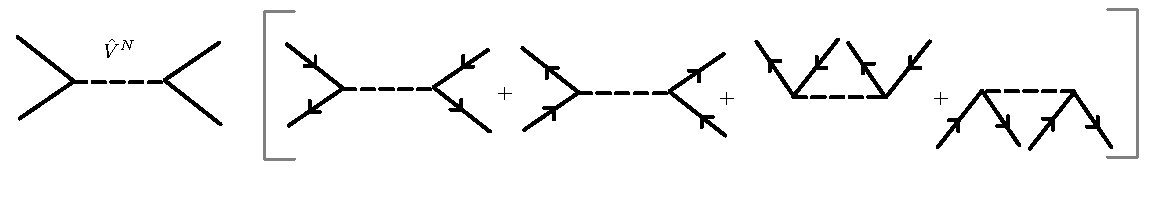
\includegraphics[width=0.99\linewidth]{VN.pdf}
        \caption{The normal ordered potential in diagrammatic form. To the left, we have the general operator without any contractions (no arrows on lines). In the gray square bracket, the possible forms of contractions are shown where no pairs are broken.}
        \label[fig]{fig:VN}
    \end{figure}

    \begin{figure}[H]
        \centering
        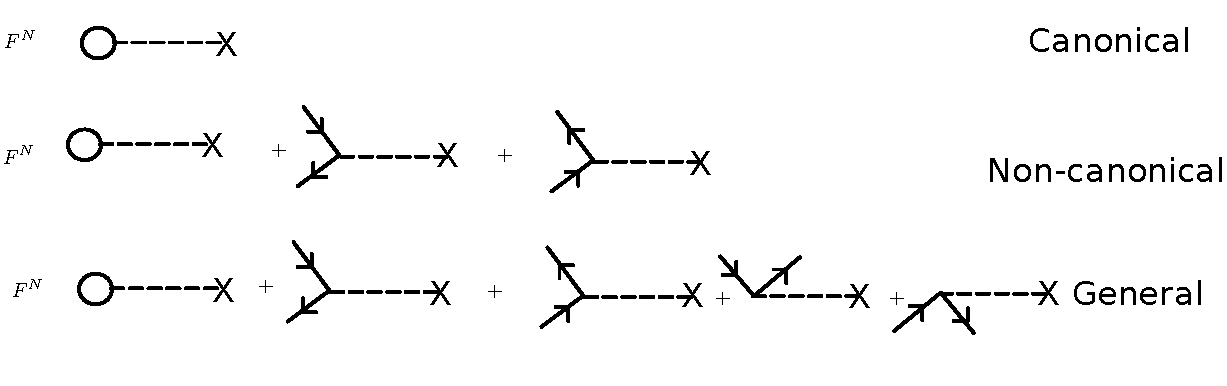
\includegraphics[width=0.99\linewidth]{FN.pdf}
        \caption{The normal ordered Fock operator for the canonical, non-canonical and general case. }
        \label[fig]{fig:FN}
    \end{figure}

\section*{Task 5}
    We now aim to solve the Hartree-Fock equations by variation of coefficient (canonical case). These equations were derived in the first midterm and in lectures, thus the Hartree-Fock matrix $\hatreefock{h}_{\alpha\beta}$ and the Hartree-Fock eigenvalue problem will only be presented here.

    \begin{align*}
        \hatreefock{h}_{\alpha\beta} &= \inner{\alpha}{\hat{h}_0}{\beta} + \sum_j \sum_{\gamma\delta} C_{j\gamma}^* C_{j\delta} \inner{\alpha\gamma}{V}{\beta\delta}  \\
        \sum_\beta \hatreefock{h}_{\alpha\beta}C_{i\beta} &= \hatreefock{\epsilon}_i C_{i\alpha}   
    \end{align*}
    Investigating $\hatreefock{h}_{\alpha\beta}$, we see that due to the orthonormal basis, the one body $\hat{h}_0$ is simply a Kronecker delta contributing the one body energies to the diagonal, $(\alpha-1)\delta_{\alpha\beta}$. The coefficients can be merged by the sum over $j$, defining the density matrix. By the normal initial guess $C_{i\alpha}^* = \delta_{i\alpha}$, we find it to be the $8 \times 8$ matrix we expect:
    
    \begin{align*}
        \rho_{\gamma\delta}^{(0)} = \sum_j C_{j\gamma}^* C_{j\delta} = \sum_j \delta_{j\gamma}\delta_{j\delta} \Rightarrow \rho^{(0)} = \begin{pmatrix}
            I_{4 \times 4} & 0 \\
            0 & 0 
        \end{pmatrix}
    \end{align*}
    The two body matrix elements from $\hatreefock{h}_{\alpha\beta}$ can also be reduced due to our constraints. Writing $\alpha = \set{e_\alpha, \sigma_\alpha}$ with $e_\alpha$ giving the energy level and $\sigma_\alpha$ the spin, the $\gamma\delta$ sum is actually a sum over four quantum numbers. We only get contributions from states in the same energy level, giving $e_\alpha = e_\gamma$ and $e_\beta = e_\gamma$. In addition, the spins has to couple, giving $\sigma_\alpha \neq \sigma_\gamma$ and $\sigma_\beta \neq \sigma_\delta$. Writing coupled spins as $\bar{\sigma}_\alpha = -\sigma_\alpha$, we find that the two body matrix elements also only give contributions to the diagonal of $\hatreefock{h}_{\alpha\beta}$. 

    \begin{align*}
        \sum_{\gamma\delta} \rho_{\gamma\delta} \inner{\alpha\gamma}{V}{\beta\gamma} &= \sum_{e_\gamma e_\gamma} \sum_{\sigma_\gamma \sigma_\delta} \rho_{\gamma\delta} \inner{e_\alpha \sigma_\alpha, e_\gamma\sigma_\gamma}{V}{e_\beta \sigma_\beta, e_\gamma \sigma_\delta} \\
        &= \rho_{\alpha\beta} \inner{e_\alpha \sigma_\alpha, e_\alpha \bar{\sigma}_\alpha}{V}{e_\beta \sigma_\beta, e_\beta \bar{\sigma}_\beta} = -\frac{1}{2}g \rho_{\alpha\beta} 
    \end{align*}
    With an appropriate mapping for the density matrix $\gamma, \delta \leftrightarrow e_\gamma \sigma_\delta, e_\delta \sigma_\delta$. By constructing the Hartree-Fock matrix $\hatreefock{h}_{\alpha\beta}$ with rows and columns starting with the lowest energy levels $e_\alpha = 1, \ldots 4$ and alternating spins $\sigma_\alpha = +, -, \ldots , -$ the $8 \times 8$ matrix has single particle states as rows and columns in the order: $\ket{1+}, \ket{1-}, \ket{2+}, \ket{2-}, \ket{3+}, \ket{3-}, \ket{4+}, \ket{4-}$. Since we have the clever guess of $C = I$, we find that the Hartree-Fock matrix is diagonal with the appropriate single particle energies as entries, with the addition of an interaction term of $-g/2$ for the occupied states. Then since both $\hatreefock{h}$ is diagonal and $C$ is diagonal, the eigenvalue problem is already solved! That is, we are already in a Hartree-Fock basis. This can also be seen by interpreting the Hartree-Fock approximation as a change of basis that sets ground state-1p1h interactions to zero, $\inner{\Phi_0}{H}{\Phi_i^a} = \inner{i}{f}{a} = 0$. Since our interaction only works between pairs, we already have $\inner{\Phi_0}{H}{\Phi_i^a} = 0$ and no iterative Hartree-Fock approach is necessary. Pretty neat indeed. The energy can then be evaluated by:
    
    \begin{align*}
        E[\Phi_0] = E[\hatreefock{\Phi}_0] = \sum_i \inner{i}{\hat{h}_0}{i} + \frac{1}{2}\sum_{ij}\inner{ij}{V}{ij} = 2 - g
    \end{align*}
    This is plotted and compared with the FCI calculations in \cref{fig:HF} and \cref{fig:FCI_HF_diff}. The structure of the Hartree-Fock energy is very simple in comparison with FCI, where it is simply linear in $g$, while being exact in the non-interacting $g = 0$ case. It is now clear that the potential changes the ground state energy more for $g > 0$ than $g < 0$. This can be seen by considering the energy difference between $g = 0$ and $g = \pm 0.5$. Since $V$ only gives a non-zero interaction when a 2p2h or 4p4h states are involved, the Hartree-Fock approach might not be the best choice in this case. 

    \begin{figure}[H]
        \begin{subfigure}{.49\textwidth}
            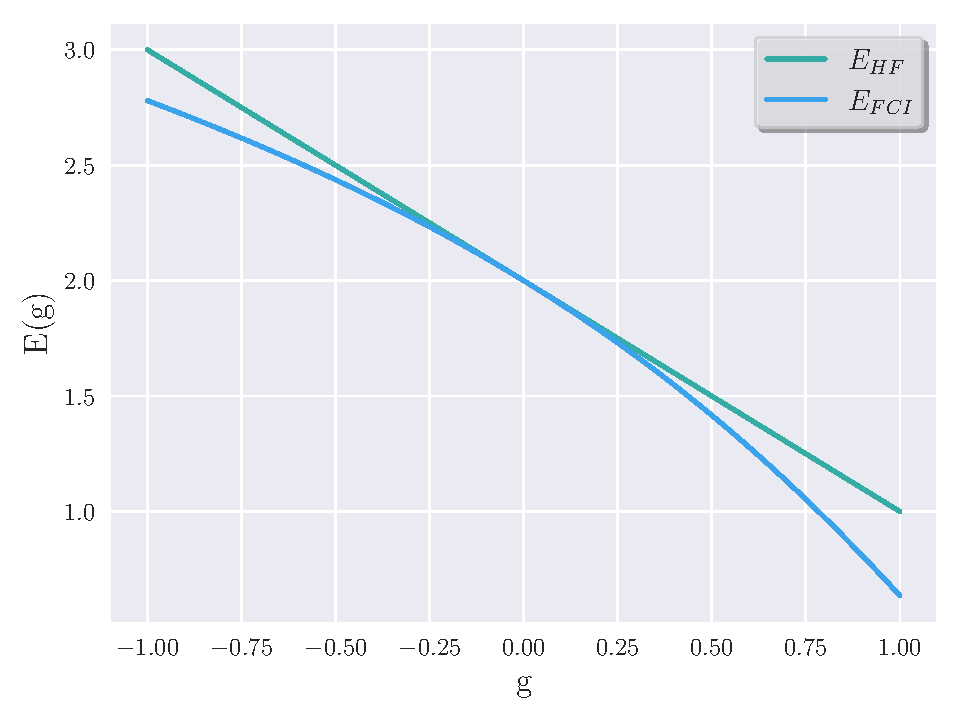
\includegraphics[width=\linewidth]{HF.pdf}
            \caption{Energy of the ground state for a Hartree Fock and FCI calculation as a function of the coupling strength $g$.}
        \label[fig]{fig:HF}
        \end{subfigure}
        \hfill
        \begin{subfigure}{.49\textwidth}
            \centering
            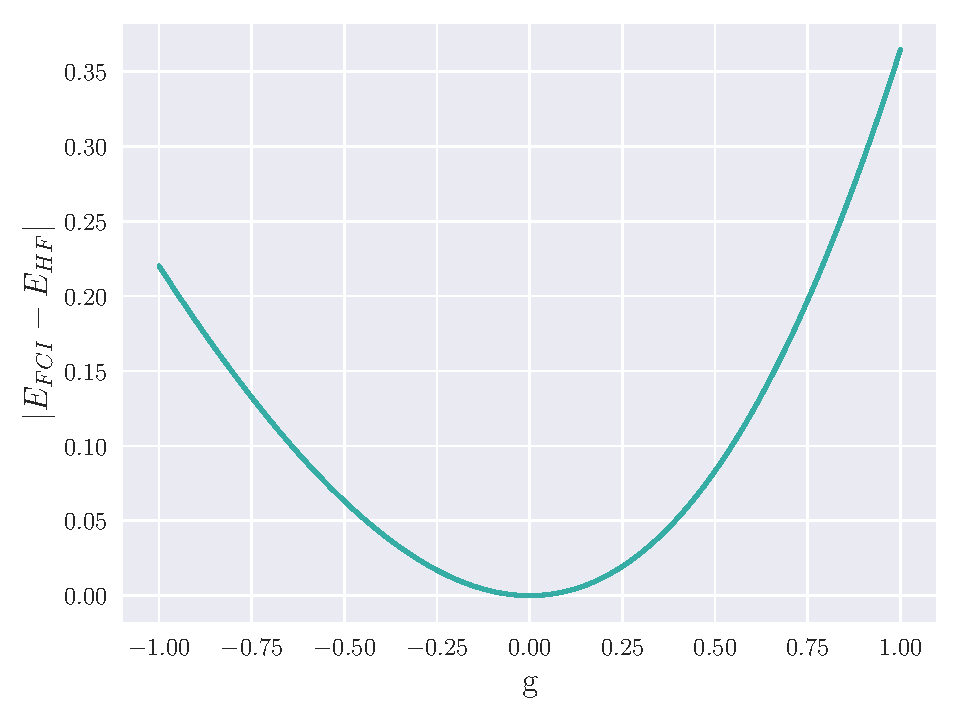
\includegraphics[width=\linewidth]{FCI_HF_diff.pdf}
            \caption{Absolute difference between ground state energies calculated using FCI and Hartree Fock as a function of coupling strength $g$}
            \label[fig]{fig:FCI_HF_diff}
        \end{subfigure}
        \caption{Hartree-Fock calculations compared with FCI}
    \end{figure}
    We now on to many body perturbation theory. The ground state energy is expanded in a perturbative series, where the (not guaranteed) goal is to converged to the true energy (FCI) for the space you are working in. Terms are summed order by order, where we first consider perturbation theory to third order in the interaction (how many $\hat{V}$ factors to include). This can be expressed as:
    
    \begin{align*}
        \ord{E}{3}_{RS} &= \ord{E}{0} + \ord{E}{1} + \ord{E}{2} + \ord{E}{3} \\ 
        \ord{E}{0} &= \inner{\Phi_0}{\hat{H}_0}{\Phi_0} = 2 \\
        \ord{E}{1} &= \inner{\Phi_0}{V}{\Phi_0} = -g \\
        \ord{E}{2} &= \psum_{i} \frac{V_{0i}V_{i0}}{D_{0i}} \\
        \ord{E}{3} &= \psum_{ij} \frac{V_{0i}W_{ij}V_{j0}}{D_{0i}D_{0j}}
    \end{align*}
    Where we have quite a lot of shorthand notation. Firstly, the sum over $i$ and $ij$ does not refer to states under the Fermi level, but rather every possible Slater determinant we can create in our space, that is the states presented in Task 2. The prime indicates that the ground state should \textit{not} be included in the sum, it only runs over excited states. In the denominator of $\ord{E}{2}$ and $\ord{E}{3}$ we have energy differences, that is with $\ord{E}{0}_i = \inner{\Phi_i}{\hat{H}_0}{\Phi_i}$ where $\ket{\Phi_i}$ as one of the excited states, $D_{0i} = \ord{E}{0}_0 - \ord{E}{0}_i$. The $V$'s with subscripts are transition probabilities, where $V_{ij} = \inner{\Phi_i}{\hat{V}}{\Phi_j}$ For $\ord{E}{3}$ we also have $W$ with subscripts. This is a transition probability with the addition of diagonal contributions from $\ord{E}{1}$, $W_{ij} = V_{ij} - \delta_{ij}\ord{E}{1}$. We observe that including $\ord{E}{0}$ and $\ord{E}{1}$ yields our results from the Hartree Fock calculations, $2-g$- 
    
    Based on the anti-symmetric Goldstone diagrams in Figure 2. from the task sheet, there are many 2nd and 3rd order contribution for a general Hamiltonian. However, since we only have paired states, and the interaction only works between pairs, there can only be 2p2h contributions. This leaves only contributions from diagram 1 for 2nd order. However, for 3rd order, we have the possible 3, 4, 5, 8 and 9 diagrams. Diagram 3 breaks a pair, and can thus not contribute.  

    Based on the second order diagram that contributes \cref{fig:diag_ord_2}, we read of the explicit contribution using the diagram rules. We have $n_h = 2$ hole lines and $n_l = 2$ loops, giving a phase factor of $(-1)^0 = 1$. In addition, we have $n_e = 2$ equivalent line pairs connecting to the same two vertices in the same direction. 
    \begin{align*}
        \text{Diagram 1}& = \frac{1}{4} \sum_{abij} \frac{\inner{ij}{V}{ab}\inner{ab}{V}{ij}}{\epsilon_i + \epsilon_j - \epsilon_a - \epsilon_b} \\
            &= \frac{1}{4}\sum_{e_a e_i}\sum_{\sigma_i \sigma_a} \frac{|\inner{e_i\sigma_i, e_i\bar{\sigma}_i}{V}{e_a\sigma_a, e_a\bar{\sigma}_a}|^2}{2\epsilon_i - 2\epsilon_a} = \frac{1}{4}\sum_{ai} \frac{4(-g/2)^2}{2(\epsilon_i-\epsilon_a)} = \frac{1}{8}\sum_{ai} \frac{g^2}{i-a}
    \end{align*}
    The notation for indices above might be confusing, but it can be viewed as follows. The first equality has sums over both quantum numbers $i = \set{e_i, \sigma_i}$, energy level and spin. This is then expanded into explicit energy level and spin indices, $e_i, \sigma_i$, with the notation $\bar{\sigma}_i = -\sigma_i$. Thereafter, since the sum over spin only gives $-g/2$ (with a factor in front, $1$ or $2$), we go back to the notation $i = e_i$, representing only the energy level. I am sorry this is confusing, but otherwise I think it would look pretty cluttered. The third order diagrams that contribute are shown in \cref{fig:diag_ord_3_45}, \cref{fig:diag_ord_3_89} and \cref{fig:diag_ord_3_unlinked}. Diagrams 4 and 5, both have $n_e = 3$ equivalent pairs, giving a factor $1/8$. Again both have $n_l = 2$ loops but $n_h = 2$ and $n_h = 4$ hole lines respectively. This however, yields the same phase factor of $(-1)^2 = (-1)^0 = 1$. By the same methodology as above, the contributions can be written as: 
    \begin{align*}
        \text{Diagram 4} &= \frac{1}{8} \sum_{abcdij} \frac{\inner{ij}{V}{ab}\inner{ab}{V}{cd}\inner{cd}{V}{ij}}{(\epsilon_i + \epsilon_j - \epsilon_a - \epsilon_b)(\epsilon_i + \epsilon_j - \epsilon_c - \epsilon_d)} = -\frac{1}{32}\sum_{iac}\frac{g^3}{(i-a)(i-c)}\\
        \text{Diagram 5} &= \frac{1}{8} \sum_{abijkl} \frac{\inner{ij}{V}{ab}\inner{kl}{V}{ij}\inner{ab}{V}{kl}}{(\epsilon_i + \epsilon_j - \epsilon_a - \epsilon_b)(\epsilon_k + \epsilon_l - \epsilon_a - \epsilon_b)} = -\frac{1}{32}\sum_{ika}\frac{g^3}{(i-a)(k-a)}
    \end{align*}
    We also have contributions from diagrams 8 and 9. Here we have $n_e = 1$ and $n_l = 3$ loops. In addition, with $n_h = 4, 2$ for 8 and 9 respectively, we get the same phase factor of $-1$. Using general indices and then applying what we know about the form of the matrix elements, we end up with:  

    \begin{align*}
        \text{Diagram 8} &= -\frac{1}{2}\sum_{abijkl} \frac{\inner{ij}{V}{ab}\inner{kl}{V}{ki}\inner{ab}{V}{lj}}{(\epsilon_i + \epsilon_j - \epsilon_a - \epsilon_b)(\epsilon_i + \epsilon_k - \epsilon_a - \epsilon_b)} = \frac{1}{16} \sum_{ia} \frac{g^3}{(i-a)^2} \\
        \text{Diagram 9} &= -\frac{1}{2} \sum_{abcdij} \frac{\inner{ij}{V}{ab}\inner{ca}{V}{cd}\inner{db}{V}{ij}}{(\epsilon_i + \epsilon_j - \epsilon_a - \epsilon_b)(\epsilon_i + \epsilon_j - \epsilon_a - \epsilon_c)} = \frac{1}{16}\sum_{ia} \frac{g^3}{(i-a)^2}
    \end{align*}
    Before we continue, we have to be a little careful. Since we are going to third order perturbation theory, the possibility for unlinked diagrams appear. From $W_{ii} = V_{ii} - \ord{E}{1}$, we have a contribution from $\ord{E}{1}$, shown in \cref{fig:diag_ord_3_unlinked}. It turns out that this luckily will exactly cancel with $V_{ii}$ (the same contribution from diagram 8/9 but with opposite sign). Writing it out we find:
    \begin{align}
         \\
        \text{3rd order unlinked} &= \sum_{ijklab} \frac{\inner{ij}{V}{ab}\inner{kl}{V}{kl}\inner{ab}{V}{ij}}{(\epsilon_i + \epsilon_j - \epsilon_a - \epsilon_b)(\epsilon_i + \epsilon_j - \epsilon_a - \epsilon_b)} = -\frac{1}{16} \sum_{ia} \frac{g^3}{(i-a)^2}   
    \end{align}

    Now, by using Diagram 1, 4, 5, 8 and 9 we calculate the perturbation energy to 3rd order, $\ord{E}{3}_{RS}$. This is compared with the FCI calculations in figure \cref{fig:RS3} and \cref{fig:FCI_RS3_diff}. We note that comparing the absolute difference for CI \cref{fig:FCI_CID_diff} and RS3 \cref{fig:FCI_RS3_diff} the error is on the same order of magnitude. The trend we have seen so far by having a larger error for $g > 0$ seems not to be the case for RS3. Perturbation theory has no guarantee for convergence and the results can vary across different orders. In this case (it is a little hard to make out from the figure) it actually crosses the energy line from FCI, giving a larger/smaller energy depending on the sign of $g$. 

    \begin{figure}[H]
        \begin{subfigure}{.49\textwidth}
            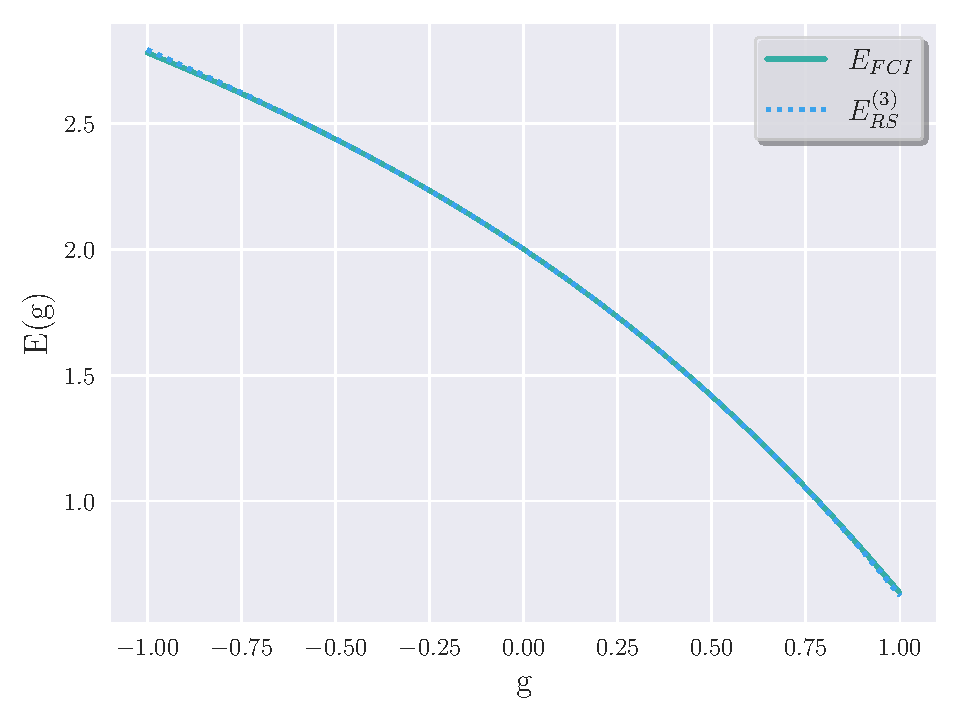
\includegraphics[width=\linewidth]{RS3.pdf}
            \caption{Energy of the ground state for a 3rd order perturbation and FCI calculation as a function of the coupling strength $g$. Qualitatively, the two lines overlap for all $g$.}
        \label[fig]{fig:RS3}
        \end{subfigure}
        \hfill
        \begin{subfigure}{.49\textwidth}
            \centering
            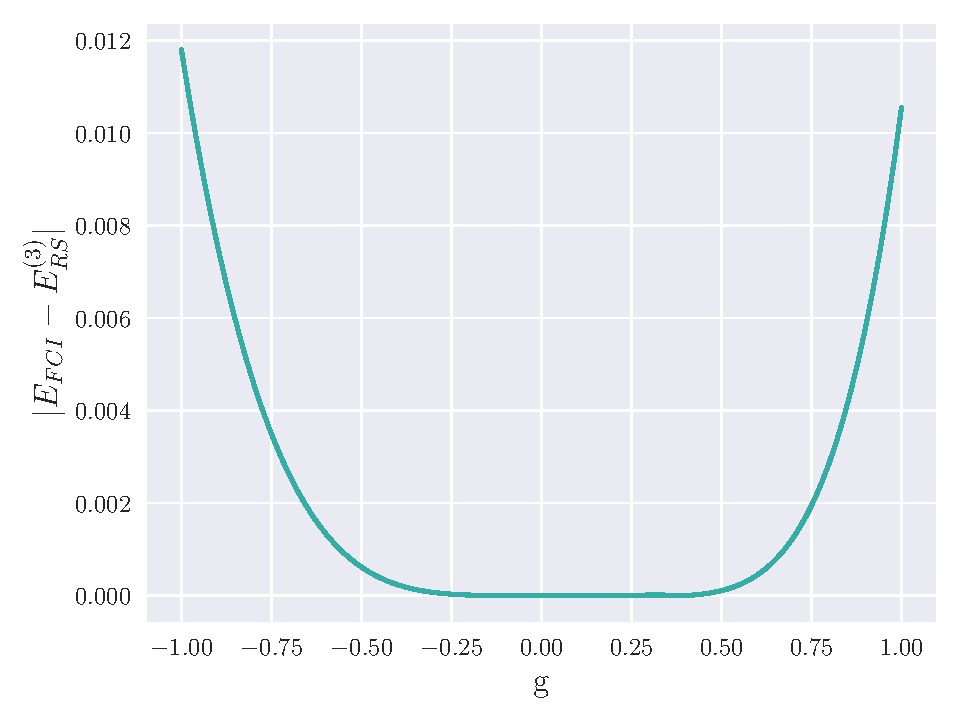
\includegraphics[width=\linewidth]{FCI_RS3_diff.pdf}
            \caption{Absolute difference between ground state energies calculated using FCI and 3rd order perturbation theory as a function of coupling strength $g$}
            \label[fig]{fig:FCI_RS3_diff}
        \end{subfigure}
        \caption{Perturbation theory to third order in the interaction, compared with FCI}
    \end{figure}

    \begin{figure}[H]
        \centering
        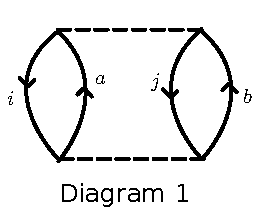
\includegraphics[width=0.33\linewidth]{diag1.pdf}
        \caption{Diagram containing second order interaction. The naming follows the task sheet and the general indices refer to both energy level and spin quantum numbers.}
        \label[fig]{fig:diag_ord_2}
    \end{figure}

    \begin{figure}[H]
        \centering
        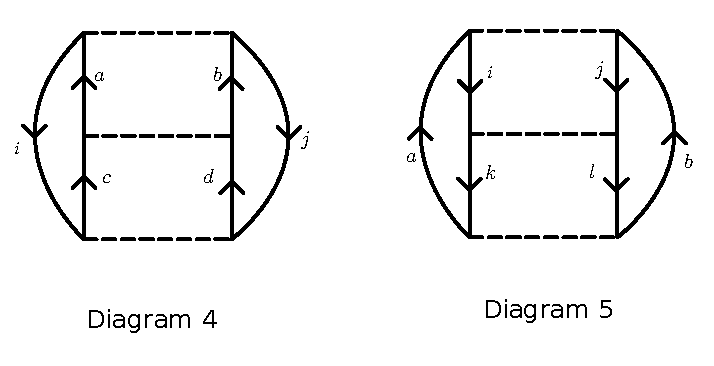
\includegraphics[width=0.8\linewidth]{diag45.pdf}
        \caption{Two diagrams giving contributions to third order. The naming follows the task sheet and the general indices refer to both energy level and spin quantum numbers.} 
        \label[fig]{fig:diag_ord_3_45}
    \end{figure}

    \begin{figure}[H]
        \centering
        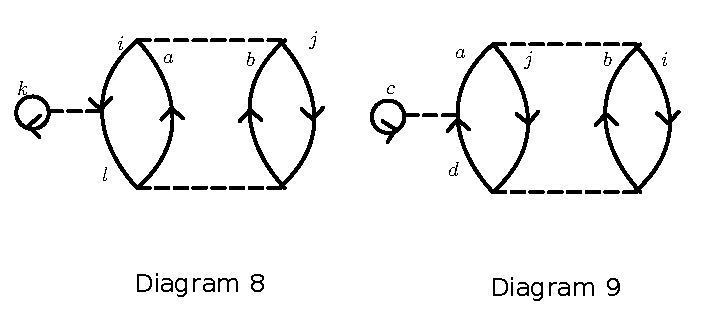
\includegraphics[width=0.8\linewidth]{diag89.pdf}
        \caption{Two diagrams giving contributions to third order. The naming follows the task sheet and the general indices refer to both energy level and spin quantum numbers.} 
        \label[fig]{fig:diag_ord_3_89}
    \end{figure}

    \begin{figure}[H]
        \centering
        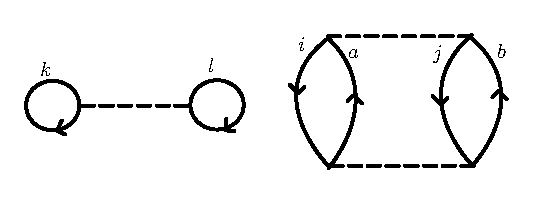
\includegraphics[width=0.8\linewidth]{diagunlinked.pdf}
        \caption{Unlinked diagram from $W_{ii}$ to third order in perturbation theory. General indices refer to both energy level and spin quantum numbers.} 
        \label[fig]{fig:diag_ord_3_unlinked}
    \end{figure}


\section*{Task 6}
    We now express the wave operator for second order in the interaction. By applying this operator on our ground state ansatz, we aim to achieve a better approximation for the true ground state by expanding it using the excited states. The inner product between the ground state and excited states, scaled by the sum of single particle energies, gives the coefficients for this expansion. We write this as:  
    \begin{align*}
        \ord{\Omega}{1} \ket{\Phi_0} = \psum_m \ket{\Phi_m} \frac{\inner{\Phi_m}{\hat{V}}{\Phi_0}}{\ord{E}{0} - \ord{E}{0}_i} = \sum_{IA} \exed{I}{A} \frac{\inner{\Phi_I^A}{\hat{V}}{\Phi_0}}{\ord{E}{0} - \ord{E}{0}_{IA}}  
    \end{align*}
    Again, here $I$ and $A$ refers to a pair of states with oppositely aligned spin. The energy to second order can be found by considering the inner product.
    
    \begin{align*}
        \ord{E}{2}_{RS} = \inner{\Phi_0}{\hat{V}\ord{\Omega}{2}}{\Phi_0}
    \end{align*}
    A comparison between second order perturbation theory and the CI calculations is presented in \cref{fig:RS2} and \cref{fig:CI_RS2_diff}. The characteristics here are similar to what we found for third order (\cref{fig:RS3} and \cref{fig:FCI_RS3_diff}), but the approximation is worse. Therefor, the addition of third order terms does yield a better result. Again we see fluctuations being both over and under the CI energy for different values of $g$ (shifting with the sign). 
    \begin{figure}[H]
        \begin{subfigure}{.49\textwidth}
            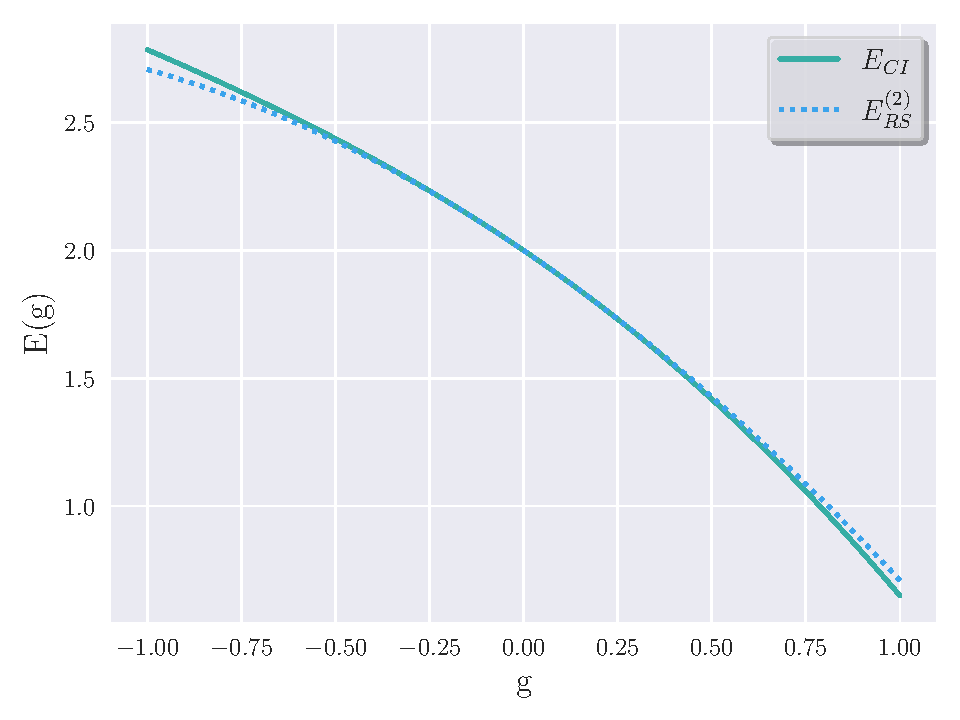
\includegraphics[width=\linewidth]{RS2.pdf}
            \caption{Energy of the ground state for a second order perturbation and CI calculation as a function of the coupling strength $g$.}
        \label[fig]{fig:RS2}
        \end{subfigure}
        \hfill
        \begin{subfigure}{.49\textwidth}
            \centering
            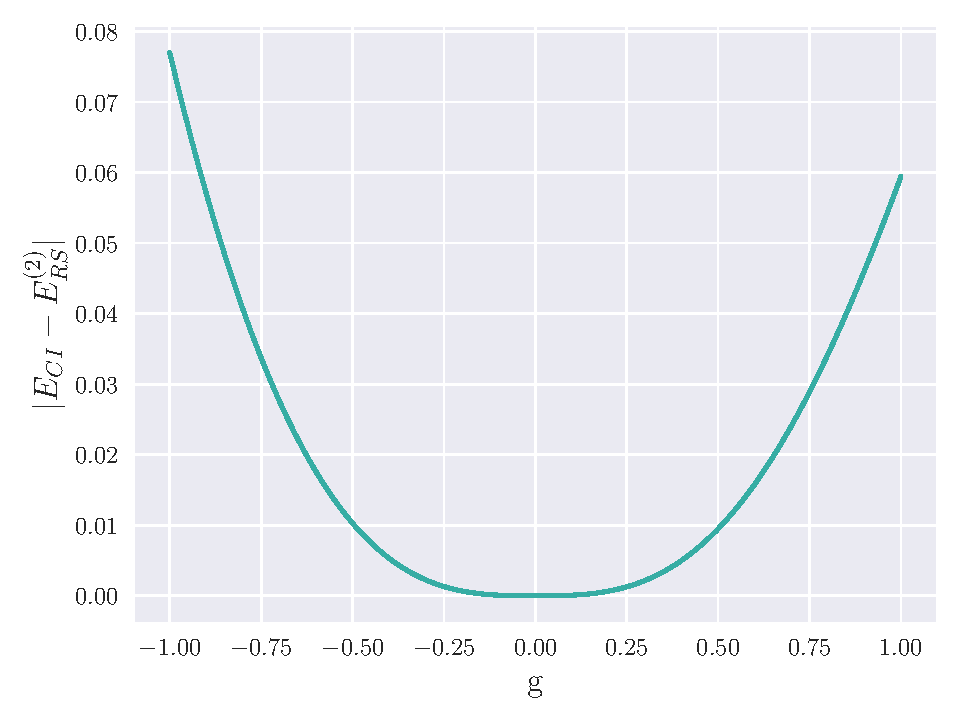
\includegraphics[width=\linewidth]{CI_RS2_diff.pdf}
            \caption{Absolute difference between ground state energies calculated using CI and second order perturbation theory as a function of coupling strength $g$.}
            \label[fig]{fig:CI_RS2_diff}
        \end{subfigure}
        \caption{Perturbation theory to second order in the interaction, compared with CI}
    \end{figure}

\section*{Task 7}
Diagrams can be separated into two categories, \textit{linked} and \textit{unlinked}. Linked diagrams have every interaction vertex linked together through either particle or hole lines. That is, the diagram can not be partitioned into smaller, lower order diagrams. Unlinked diagrams on the other hand, have at least two interaction pieces that does not link together, meaning that the diagrams can be separated into more than one lower order diagram. These diagrams give nonphysical dependence on the number of particles in the system, leading to the possibility that the system is not size extensive. Goldstone's linked diagram theorem proves that these nonphysical diagrams cancel order by order, provided that the complete diagrams are evaluated.

Regarding diagrams, the 1p1h fourth order diagrams can not contribute as they break a pair. The 2p2h diagrams on the other hand is harder to make out, they all sort of look the same. An (un)educated guess would be 14 and 15. One of these (or some other contributing diagram) would presumably cancel a first times third order diagram and two second order diagrams. However, the contribution can be calculated by adding:

\begin{align*}
    \ord{E}{4}_{RS} = \ord{E}{3}_{RS} + \psum_{ijk} \frac{V_{0i}W_{ij}W_{jk}V_{k0}}{D_{0i}D_{0j}D_{0k}} - \ord{E}{2} \psum_{i} \frac{V_{0i}V_{i0}}{D_{0i}^2}
\end{align*}


The results for perturbation theory to the fourth order in the interaction is presented in \cref{fig:RS3} and \cref{fig:FCI_RS3_diff}. Compared with the result from third order (\cref{fig:RS3}, \cref{fig:FCI_RS3_diff}), the improvements are very small where present. Due to the fluctuations previously mentioned, we now have a larger error for $g > 0$ again (which was different for third order). Just as in the third order case, the energy fluctuates as a function of $g$, being above for $g < 0$ and below for $g > 0$. 

\begin{figure}[H]
    \begin{subfigure}{.49\textwidth}
        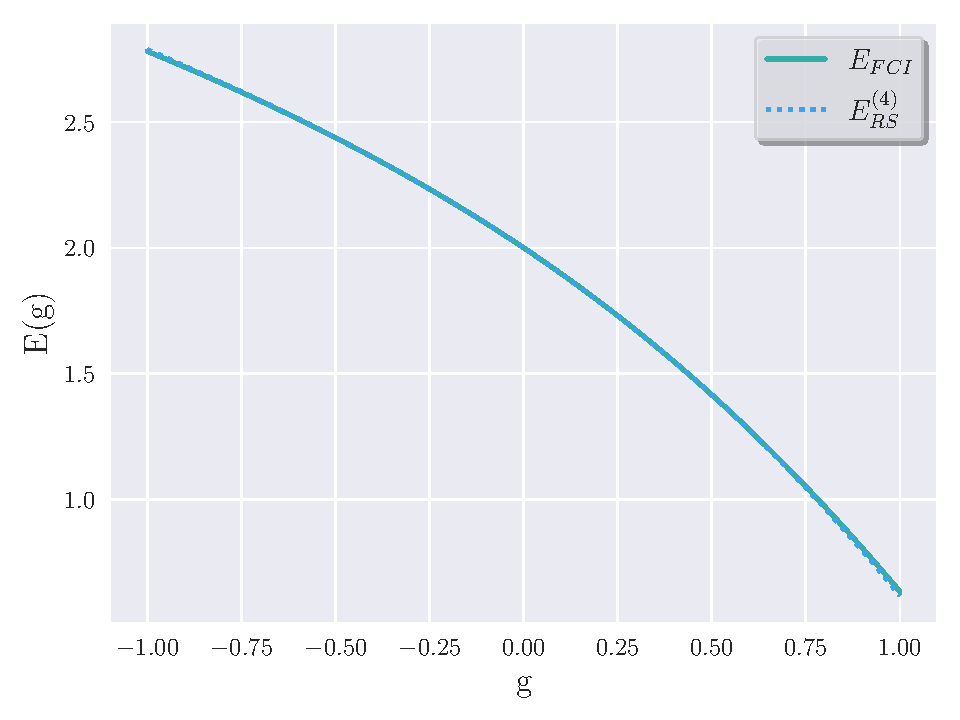
\includegraphics[width=\linewidth]{RS4.pdf}
        \caption{Energy of the ground state for a foruth order perturbation and FCI calculation as a function of the coupling strength $g$.}
    \label[fig]{fig:RS4}
    \end{subfigure}
    \hfill
    \begin{subfigure}{.49\textwidth}
        \centering
        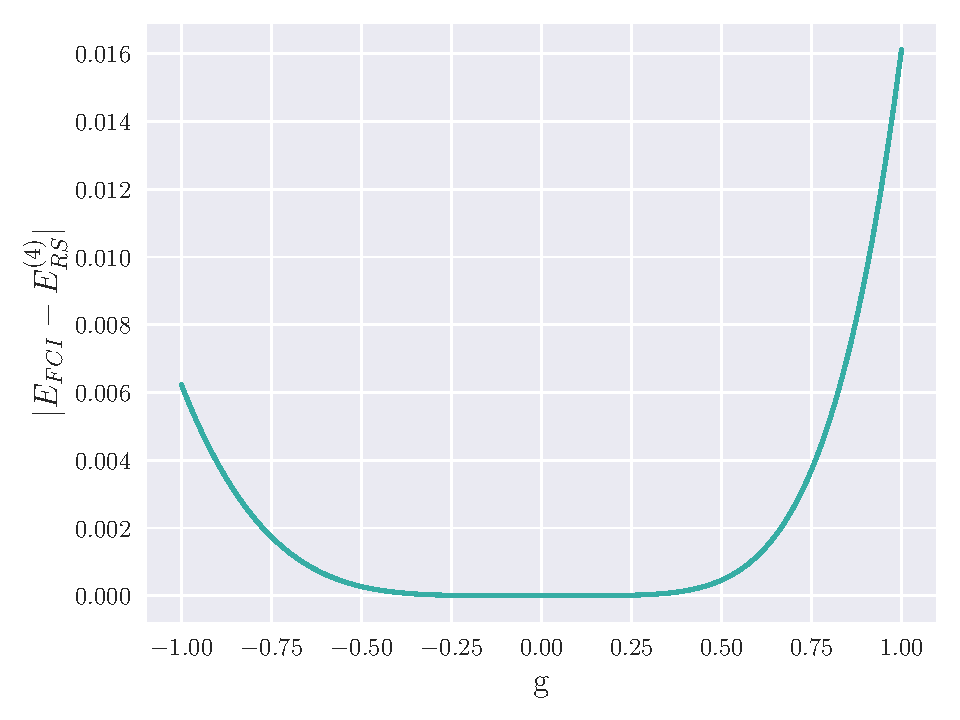
\includegraphics[width=\linewidth]{FCI_RS4_diff.pdf}
        \caption{Absolute difference between ground state energies calculated using FCI and foruth order perturbation theory as a function of coupling strength $g$.}
        \label[fig]{fig:FCI_RS4_diff}
    \end{subfigure}
    \caption{Perturbation theory to second order in the interaction, compared with CI}
\end{figure}

\printbibliography

\end{document}
